%_______________________________________________________________________________
\section{Description des paquets scientifiques}
%_______________________________________________________________________________
%_______________________________________________________________________________
\begin{frame}[fragile]
\frametitle{Quelques Paquets et Outils Scientifiques}
\begin{itemize}
 \item SciPy : scientific python 
 \begin{itemize}
  \item Numpy
  \item SciPy library
  \item Matplotlib
  \item IPython
 \end{itemize}
 \item Mayavi : objets 3D avancés
 \item Scikit-learn : machine learning.
 \item \dots
\end{itemize}
\end{frame}
%_______________________________________________________________________________
%_______________________________________________________________________________
\subsection{SciPy}
%_______________________________________________________________________________
%_______________________________________________________________________________
\begin{frame}[fragile]
\frametitle{SciPy}
\framesubtitle{}
\begin{itemize}
 \item \url{http://www.scipy.org/}
\end{itemize}
\begin{center}
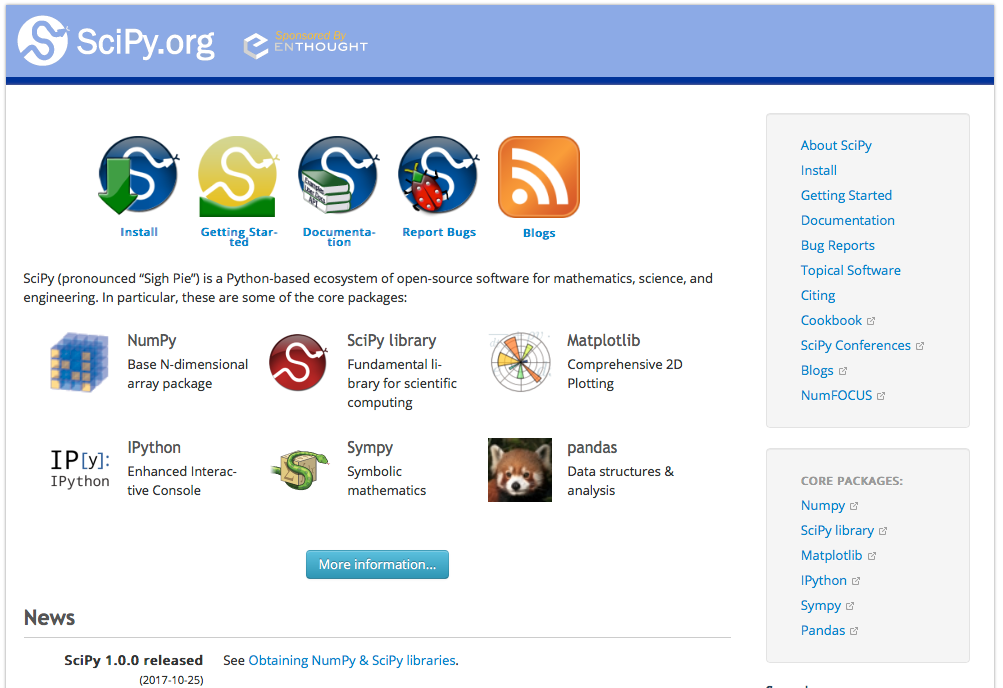
\includegraphics[width=10cm]{./fig/scipy.png}
\end{center}
\end{frame}
%_______________________________________________________________________________
%_______________________________________________________________________________
\subsection{Numpy}
%_______________________________________________________________________________
%_______________________________________________________________________________
\begin{frame}[fragile]
\frametitle{Numpy}
\begin{itemize}
 \item \myFig{height=0.5cm}{./fig/numpy-logo.png} \, \url{http://www.numpy.org}
 \item \emph{NumPy is the fundamental package for scientific computing with Python}
\end{itemize}
\begin{pythonConsole}
>>> import numpy
>>> help(numpy)

Help on package numpy:

NAME
    numpy

FILE
    /Users/becqg/Library/Enthought/Canopy_64bit/User/lib/python2.7/site-packages
    /numpy/__init__.py

DESCRIPTION
    NumPy
    =====
    
    Provides
      1. An array object of arbitrary homogeneous items
      2. Fast mathematical operations over arrays
      3. Linear Algebra, Fourier Transforms, Random Number Generation
    
...
\end{pythonConsole}
\end{frame}
%_______________________________________________________________________________
%_______________________________________________________________________________
\subsubsection{ndarray}
%_______________________________________________________________________________
%_______________________________________________________________________________
\begin{frame}[fragile]
\frametitle{N-dimensional array Object}
\framesubtitle{}
\begin{itemize}
 \item N-dimensional array : ndarray
 \item Création d'un tableau vide et réservation de l'espace (empty)
 \item Accès aux éléments : A[i, j, \dots] 
 \item indices de {\color{red}{0 à $n-1$}}
 \item indices négatifs de $-n$ à $-1$
\end{itemize}
\begin{pythonConsole}

>>> A = numpy.empty((2, 2))
>>> print(A)
[[ -1.28822975e-231   2.68678092e+154]
 [  2.24497156e-314   2.24499315e-314]]
>>> A[0, 0] = 1
>>> A[1, 0] = 2
>>> A[0, 1] = 11
>>> A[1, 1] = 12
>>> print(A)
[[  1.   2.]
 [ 11.  12.]]
>>> type(A)
<type 'numpy.ndarray'>
>>> A[-1, -2] = 11
\end{pythonConsole}
\end{frame}
%_______________________________________________________________________________
%_______________________________________________________________________________
\begin{frame}[fragile]
\frametitle{N-dimensional array Object}
\framesubtitle{}
\begin{itemize}
 \item Rappel : accès aux propiétés et méthodes (dir) 
\end{itemize}
\begin{pythonConsole}

>>> dir(A)
'T', ..., 'all', 'any', 'argmax', 'argmin', 'argpartition', 'argsort', 'astype',
'base', 'byteswap', 'choose', 'clip', 'compress', 'conj', 'conjugate', 'copy',
'ctypes', 'cumprod', 'cumsum', 'data', 'diagonal', 'dot', 'dtype', 'dump',
'dumps', 'fill', 'flags', 'flat', 'flatten', 'getfield', 'imag', 'item',
'itemset', 'itemsize', 'max', 'mean', 'min', 'nbytes', 'ndim', 'newbyteorder',
'nonzero', 'partition', 'prod', 'ptp', 'put', 'ravel', 'real', 'repeat',
'reshape', 'resize', 'round', 'searchsorted', 'setfield', 'setflags', 'shape',
'size', 'sort', 'squeeze', 'std', 'strides', 'sum', 'swapaxes', 'take',
'tofile', 'tolist', 'tostring', 'trace', 'transpose', 'var', 'view'
\end{pythonConsole}
\end{frame}
%_______________________________________________________________________________
%_______________________________________________________________________________
\begin{frame}[fragile]
\frametitle{N-dimensional array Object}
\framesubtitle{Attributs sur la forme du tableau}
\begin{itemize}
 \item Forme du tableau (shape), c'est un tuple.  
 \item Nombre de dimension (ndim)
 \item Type des éléments (dtype)
 \item Taille du tableau (size), c'est le nombre de cellules totales. 
\end{itemize}
\begin{pythonConsole}
>>> A.shape
(2, 2)
>>> (nRow, nCol) = A.shape
>>> nRow = A.shape[0]
>>> nCol = A.shape[1]
>>> A.ndim
2
>>> A.dtype
dtype('float64')
>>> A.size
4
\end{pythonConsole}
\end{frame}
%_______________________________________________________________________________
%_______________________________________________________________________________
\begin{frame}[fragile]
\frametitle{N-dimensional array Object}
\framesubtitle{Changement de forme}
\begin{itemize}
 \item Pour changer la forme (reshape)
 \item Transposition (T)
\end{itemize}
\begin{pythonConsole}
>>> B = A.reshape((4, 1))
array([[  1.],
       [  2.],
       [ 11.],
       [ 12.]])
>>> B.ndim
2
>>> B.size
4
>>> B.T
array([[ 1.,   2.,  11.,  12.]])
\end{pythonConsole}
\end{frame}
%_______________________________________________________________________________
%_______________________________________________________________________________
\begin{frame}[fragile]
\frametitle{N-dimensional array Object}
\framesubtitle{Copie de tableaux}
\begin{itemize}
 \item Les éléments de B sont les mêmes que ceux de A, seule la forme change. 
 \item Si on veut une copie (copy)
\end{itemize}
\begin{pythonConsole}
>>> B[0, 0] = 21
>>> print(A)
[[ 21.   2.]
 [ 11.  12.]]
>>> B[1, 0]
>>> C = A.copy()
>>> C[0, 0] = 31
>>> print(A[0,0], C[0,0])
(21.0, 31.0)
\end{pythonConsole}
\end{frame}
%_______________________________________________________________________________
%_______________________________________________________________________________
\begin{frame}[fragile]
\frametitle{N-dimensional array Object}
\framesubtitle{Création de tableaux}
\begin{itemize}
 \item tableau vide et réservation de l'espace (empty)
 \item initialisation à zeros (zeros)
 \item initialisation avec des uns (ones)
 \item tableau identité (eye) avec la dimension. 
 \item à partir de listes (array)
 \item suivant une étendue (arange)
\end{itemize}
\begin{pythonConsole}
>>> A = numpy.zeros((2, 4))
>>> print(A)
[[ 0.  0.  0.  0.]
 [ 0.  0.  0.  0.]]
>>> A = numpy.ones((3, 2))
>>> print(A)
[[ 1.  1.]
 [ 1.  1.]
 [ 1.  1.]]
>>> A = numpy.eye(2)
>>> print(A)
[[ 1.  0.]
 [ 0.  1.]]
>>> A = numpy.array([[1, 2], [11, 12]])
>>> print(A)
[[ 1  2]
 [11 12]]
>>> print(numpy.arange(0.5, 1.7, 0.1))
[ 0.5  0.6  0.7  0.8  0.9  1.   1.1  1.2  1.3  1.4  1.5  1.6]
\end{pythonConsole}
\end{frame}
%_______________________________________________________________________________
%_______________________________________________________________________________
\begin{frame}[fragile]
\frametitle{N-dimensional array Object}
\framesubtitle{Types}
\begin{itemize}
 \item Définition du type à la création
 \item Changement de type (astype)
 \item Multiplication ou addition avec un scalaire typé. 
\end{itemize}
\begin{pythonConsole}
>>> A = numpy.array([[1, 2], [11, 12]])
>>> print(A.dtype)
int64
>>> A = numpy.array([[1., 2], [11, 12]])
>>> print(A.dtype)
float64
>>> A = numpy.array([[1, 2], [11, 12]], dtype="float")
>>> print(A.dtype)
float64
>>> A = A.astype("complex")
>>> print(A)
[[  1.+0.j   2.+0.j]
 [ 11.+0.j  12.+0.j]]
>>> A = numpy.array([[1, 2], [11, 12]]) * 1.
>>> print(A.dtype)
float64
\end{pythonConsole}
\end{frame}
%_______________________________________________________________________________
%_______________________________________________________________________________
\begin{frame}[fragile]
\frametitle{N-dimensional array Object}
\framesubtitle{Additions, soustractions, multiplications sur les tableaux}
\begin{itemize}
 \item Addition, soustraction de tableaux ou d'un scalaire (+, -)
 \item Multiplication par un scalaire (*)
 \item Produit élément par élément (*) 
\end{itemize}
\begin{pythonConsole}
>>> A = numpy.array([[1, 2], [11, 12]])
>>> B = numpy.array([[3, 4], [13, 14]])
>>> print(A + 10)
[[ 11.  12.]
 [ 21.  22.]]
>>> print(A + B)
[[  4.   6.]
 [ 24.  26.]]
>>> print(A * 10)
[[  10.   20.]
 [ 110.  120.]]
>>> print(A * B)
[[   3.    8.]
 [ 143.  168.]]
>>> C = numpy.ones((10, ))
>>> print(A * C)
Traceback (most recent call last):
  File £"£<stdin>£"£, line 1, in <module>
ValueError: operands could not be broadcast together with shapes (2,2) (10) 
\end{pythonConsole}
\end{frame}
%_______________________________________________________________________________
%_______________________________________________________________________________
\begin{frame}[fragile]
\frametitle{N-dimensional array Object}
\framesubtitle{Produit scalaire}
\begin{itemize}
 \item Produit scalaire (dot)
 \item See also numpy.dot : en général, pour chaque méthode associée à un ndarray, il existe une fonction équivalente dans numpy. 
\end{itemize}
\begin{pythonConsole}
>>> A = numpy.array([[1, 2], [11, 12]])
>>> B = numpy.array([[3, 4], [13, 14]])
>>> print(A.dot(B))
[[  29.   32.]
 [ 189.  212.]]
>>> print(numpy.dot(A, B))
[[  29.   32.]
 [ 189.  212.]]
>>> C = numpy.ones((10, ))
>>> print(A.dot(C))
Traceback (most recent call last):
  File £"£<stdin>£"£, line 1, in <module>
ValueError: matrices are not aligned
>>> 
\end{pythonConsole}
\end{frame}
%_______________________________________________________________________________
%_______________________________________________________________________________
\begin{frame}[fragile]
\frametitle{N-dimensional array Object}
\framesubtitle{Division}
\begin{itemize}
 \item Division par un scalaire (/)
 \item Division éléments par éléments (/) 
 \item Attention au type en Python 2.7 ! 
\end{itemize}
\begin{pythonConsole}
>>> A = numpy.array([[1, 2], [11, 12]])
>>> B = numpy.array([[3, 4], [13, 14]])
>>> print(A / 2)
[[0 1]
 [5 6]]
>>> print(A / B)
[[0 0]
 [0 0]]
>>> print(A / B.astype("float"))
[[ 0.33333333  0.5       ]
 [ 0.84615385  0.85714286]]
\end{pythonConsole}
\end{frame}
%_______________________________________________________________________________
%_______________________________________________________________________________
\begin{frame}[fragile]
\frametitle{N-dimensional array Object}
\framesubtitle{Autres méthodes}
\begin{itemize}
 \item max, min, sum, mean, std, cumsum, cumprod \dots sur tous les éléments ou sur une dimension particulière (kwarg axis). 
\end{itemize}
\begin{minipage}{5cm}
\begin{pythonConsole}
>>> A = numpy.ones((2, 3, 4))
>>> print(A)
[[[ 1.  1.  1.  1.]
  [ 1.  1.  1.  1.]
  [ 1.  1.  1.  1.]]

 [[ 1.  1.  1.  1.]
  [ 1.  1.  1.  1.]
  [ 1.  1.  1.  1.]]]
>>> print(A.cumsum())
[  1.   2.   3.   4.   5.   6.   7.   8.   9.  10.  11.  12.  13.  14.  15. 
  16.  17.  18.  19.  20.  21.  22.  23.  24.]
>>> print(A.cumsum(axis=0))
[[[ 1.  1.  1.  1.]
  [ 1.  1.  1.  1.]
  [ 1.  1.  1.  1.]]

 [[ 2.  2.  2.  2.]
  [ 2.  2.  2.  2.]
  [ 2.  2.  2.  2.]]]
\end{pythonConsole}
\end{minipage}
\begin{minipage}{5cm}
\begin{pythonConsole}
>>> print(A.cumsum(axis=1))
[[[ 1.  1.  1.  1.]
  [ 2.  2.  2.  2.]
  [ 3.  3.  3.  3.]]

 [[ 1.  1.  1.  1.]
  [ 2.  2.  2.  2.]
  [ 3.  3.  3.  3.]]]
>>> print(A.cumsum(2))
[[[ 1.  2.  3.  4.]
  [ 1.  2.  3.  4.]
  [ 1.  2.  3.  4.]]

 [[ 1.  2.  3.  4.]
  [ 1.  2.  3.  4.]
  [ 1.  2.  3.  4.]]]
\end{pythonConsole}
\end{minipage}
\end{frame}
%_______________________________________________________________________________
%_______________________________________________________________________________
\begin{frame}[fragile]
\frametitle{N-dimensional array Object}
\framesubtitle{Sélection de sous-tableaux}
\begin{itemize}
 \item découpage, slicing, comme pour les séquences.
\end{itemize}
\begin{pythonConsole}
>>> A = numpy.array([[1, 2, 3, 4], [11, 12, 13, 14]])
>>> print(A)
[[ 1  2  3  4]
 [11 12 13 14]]
>>> print(A[1, :])
[11 12 13 14]
>>> print(A[:, 1:3])
[[ 2  3]
 [12 13]]
\end{pythonConsole}
\end{frame}
%_______________________________________________________________________________
%_______________________________________________________________________________
\begin{frame}[fragile]
\frametitle{N-dimensional array Object}
\framesubtitle{Sélection de sous-tableaux}
\begin{itemize}
 \item Comparaison et opérateurs logiques
 \item Opérations logiques pour sélectionner des éléments (masking)
 \item Récupérer les indices (where)
\end{itemize}
\begin{pythonConsole}
>>> A = numpy.array([[1, 2, 3, 4], [11, 12, 13, 14]])
>>> print(A)
[[ 1  2  3  4]
 [11 12 13 14]]
>>> B = A > 2
>>> print(B)
[[False False  True  True]
 [ True  True  True  True]]
>>> print(A[B])
[ 3  4 11 12 13 14]
>>> indices = numpy.where(B)
>>> print(indices[0])
array([0, 0, 1, 1, 1, 1])
>>> print(indices[1])
array([2, 3, 0, 1, 2, 3])
>>> (i, j) = numpy.where(A > 2)
\end{pythonConsole}
\end{frame}
%_______________________________________________________________________________
%_______________________________________________________________________________
\begin{frame}[fragile]
\frametitle{N-dimensional array Object}
\framesubtitle{Concaténations}
\begin{itemize}
 \item Concaténation horizontale (hstack)
 \item Concaténation verticale (vstack)
 \item concatenate (concatenate, kwarg axis)
\end{itemize}
\begin{pythonConsole}
>>> A = numpy.array([[1, 2], [11, 12]])
>>> B = numpy.array([[3, 4], [13, 14]])
>>> C = numpy.vstack((A, B))
>>> print(C)
[[ 1  2]
 [11 12]
 [ 3  4]
 [13 14]]
>>> D = numpy.hstack((A, B, A, A))
>>> print(D)
[[ 1  2  3  4  1  2  1  2]
 [11 12 13 14 11 12 11 12]]
>>> E = numpy.concatenate((A, B, A, A), axis=1)
>>> print(E)
[[ 1  2  3  4  1  2  1  2]
 [11 12 13 14 11 12 11 12]]
\end{pythonConsole}
\end{frame}
%_______________________________________________________________________________
%_______________________________________________________________________________
\begin{frame}[fragile]
\frametitle{N-dimensional array Object}
\framesubtitle{Structured Arrays}
\begin{itemize}
 \item Possibilité de mettre des éléments de types différents.  
 \item Possibilité de tableaux structurés \dots
\end{itemize}
\begin{pythonConsole}
>>> A = numpy.array([["a", 1], ["b", 2]], dtype="object")
>>> print(A)
[['a' 1]
 ['b' 2]]
>>> print(A.dtype)
object

>>> A = numpy.array([(1, "abc"), (2, "def")], dtype=[("index", "int"), 
	("name", "S8")])
>>> print(A)
[(1, 'abc') (2, 'def')]
>>> A["index"]
array([1, 2])
>>> A["name"]
array(['abc', 'def'], 
      dtype='|S8')
\end{pythonConsole}
\end{frame}
%_______________________________________________________________________________
%_______________________________________________________________________________
\subsubsection{save/load}
%_______________________________________________________________________________
%_______________________________________________________________________________
\begin{frame}[fragile]
\frametitle{Sauvegarde et lecture de données}
\framesubtitle{}
\begin{itemize}
 \item Enregistrement d'un tableau (save) dans un fichier ".npy"
 \item Enregistrement compressé de plusieurs tableaux (savez) au format ".npz"
 \item Lecture (load) des fichiers ".npy", ".npz"
\end{itemize}
\begin{pythonConsole}
>>> A = numpy.array([[1, 2], [11, 12]])
>>> numpy.save("save_A", A)
>>> del(A)
>>> A = numpy.load("save_A.npy")
>>> print(A)
[[ 1  2]
 [11 12]]
>>> A = numpy.array([[1, 2], [11, 12]])
>>> B = numpy.array([[21, 22], [31, 32]])
>>> numpy.savez("save_AB", tab1=A, B=B)
>>> del(A, B)
>>> data = numpy.load("save_AB.npz")
>>> print(data["tab1"])
[[ 1  2]
 [11 12]]
>>> print(data["B"])
[[21 22]
 [31 32]]
\end{pythonConsole}
\end{frame}
%_______________________________________________________________________________
%_______________________________________________________________________________
\begin{frame}[fragile]
\frametitle{Sauvegarde et lecture de données txt}
\framesubtitle{}
\begin{itemize}
 \item Lecture de fichier texte ".txt" (load ou loadtxt) 
 \item Enregistrement (savetxt) 
\end{itemize}
\begin{pythonConsole}
>>> A = numpy.loadtxt("data.txt")
>>> A
array([[  1.,   2.,   3.,   4.,   5.],
       [ 11.,  12.,  13.,  14.,  15.],
       [ 21.,  22.,  23.,  24.,  25.]])
>>> numpy.savetxt("data.txt", A)
\end{pythonConsole}
\end{frame}
%_______________________________________________________________________________
%_______________________________________________________________________________
\subsubsection{matrix}
%_______________________________________________________________________________
%_______________________________________________________________________________
\begin{frame}[fragile]
\frametitle{Matrix}
\framesubtitle{Définition}
\begin{itemize}
 \item Classe héritée de ndarray avec ndim = 2.  
\end{itemize}
\begin{pythonConsole}
>>> help(numpy.matrix)
class matrix(numpy.ndarray)
 |  matrix(data, dtype=None, copy=True)
 |  
 |  Returns a matrix £from£ an array-like object, £or from£ a string of data.
 |  A matrix £is£ a specialized 2-D array that retains its 2-D nature
 |  through operations.  It has certain special operators, such as £`££`£*£`££`£
 |  (matrix multiplication) £and£ £`££`£**£`££`£ (matrix power).
...
\end{pythonConsole}
\end{frame}
%_______________________________________________________________________________
%_______________________________________________________________________________
\begin{frame}[fragile]
\frametitle{Matrix}
\framesubtitle{Saisie}
\begin{itemize}
 \item Saisie directe de type ndarray avec des listes imbriquées. 
 \item Possibilité de saisie type Matlab.
\end{itemize}
\begin{pythonConsole}
>>> A = numpy.matrix([[1, 2], [11, 12]])
>>> print(A)
[[ 1  2]
 [11 12]]
>>> type(A)
 <class 'numpy.matrixlib.defmatrix.matrix'>
>>> A = numpy.matrix("[1, 2, 3, 4; 11, 12, 13, 14]")
>>> print(A)
[[ 1  2  3  4]
 [11 12 13 14]]
\end{pythonConsole}
\end{frame}
%_______________________________________________________________________________
%_______________________________________________________________________________
\begin{frame}[fragile]
\frametitle{Matrix}
\framesubtitle{Multiplication et exposant}
\begin{itemize}
 \item Produit de matrices (*)
 \item Exposant de matrice (**)
\end{itemize}
\begin{pythonConsole}
>>> A = numpy.matrix([[1, 2], [11, 12]])
>>> B = numpy.matrix([[3, 4], [13, 14]])
>>> print(A * B)
[[ 29  32]
 [189 212]]
>>> print(A ** 2)
[[ 23  26]
 [143 166]]
\end{pythonConsole}
\end{frame}
%_______________________________________________________________________________
%_______________________________________________________________________________
\begin{frame}[fragile]
\frametitle{Matrix}
\framesubtitle{Opérateurs matriciels courants}
\begin{itemize}
 \item Transposition (T)
 \item Inversion (I)
 \item Opérateur Hermitien (H)
\end{itemize}
\begin{pythonConsole}
>>> A = numpy.matrix([[1, 2], [11, 12]])
>>> print(A)
[[ 1  2]
 [11 12]]
>>> print(A.T)
[[ 1 11]
 [ 2 12]]
>>> print(A.I)
print(A.I)
[[-1.2  0.2]
 [ 1.1 -0.1]]
>>> B = numpy.matrix([[1, 2+1j], [11+1j, 12]])
>>> print(B)
[[  1.+0.j   2.+1.j]
 [ 11.+1.j  12.+0.j]]
>>> print(B.H)
[[  1.-0.j  11.-1.j]
 [  2.-1.j  12.-0.j]]
\end{pythonConsole}
\end{frame}
%_______________________________________________________________________________
%_______________________________________________________________________________
\subsubsection{subpackages}
%_______________________________________________________________________________
%_______________________________________________________________________________
\begin{frame}[fragile]
\frametitle{Autres opérations d'algèbre linéaire}
\framesubtitle{Sous paquet linalg}
\begin{itemize}
 \item Interface vers Lapack (numpy.linalg)
\end{itemize}
\begin{pythonConsole}
>>> help(numpy.linalg)
...
    Linear algebra basics:
    
    - norm            Vector £or£ matrix norm
    - inv             Inverse of a square matrix
    - solve           Solve a linear system of equations
    - det             Determinant of a square matrix
    - lstsq           Solve linear least-squares problem
    - pinv            Pseudo-inverse (Moore-Penrose)...
    - matrix_power    Integer power of a square matrix
    
    Eigenvalues £and£ decompositions:
    
    - eig             Eigenvalues £and£ vectors of a square matrix
    - eigh            Eigenvalues £and£ eigenvectors of a Hermitian matrix
    - eigvals         Eigenvalues of a square matrix
    - eigvalsh        Eigenvalues of a Hermitian matrix
    - qr              QR decomposition of a matrix
    - svd             Singular value decomposition of a matrix
    - cholesky        Cholesky decomposition of a matrix
    
    Tensor operations:
    
    - tensorsolve     Solve a linear tensor equation
    - tensorinv       Calculate an inverse of a tensor
...
\end{pythonConsole}
\end{frame}
%_______________________________________________________________________________
%_______________________________________________________________________________
\begin{frame}[fragile]
\frametitle{Autres paquets de numpy}
\framesubtitle{}
\begin{pythonConsole}
>>> help(numpy)
...
    doc
        Topical documentation on broadcasting, indexing, etc.
    lib
        Basic functions used by several sub-packages.
    random
        Core Random Tools
    linalg
        Core Linear Algebra Tools
    fft
        Core FFT routines
    polynomial
        Polynomial tools
    testing
        Numpy testing tools
    f2py
        Fortran to Python Interface Generator.
    distutils
        Enhancements to distutils with support for
        Fortran compilers support and more.
...
\end{pythonConsole}
\end{frame}
%_______________________________________________________________________________
%_______________________________________________________________________________
\begin{frame}[fragile]
\frametitle{Autres paquets de numpy}
\framesubtitle{Random}
\begin{itemize}
 \item Sous paquet random : générateurs de nombres aléatoires. 
\end{itemize}
\begin{pythonConsole}
>>> numpy.random.seed(0)
>>> A = numpy.random.randn(2, 3, 4)
>>> print(A)
[[[ 1.76405235  0.40015721  0.97873798  2.2408932 ]
  [ 1.86755799 -0.97727788  0.95008842 -0.15135721]
  [-0.10321885  0.4105985   0.14404357  1.45427351]]

 [[ 0.76103773  0.12167502  0.44386323  0.33367433]
  [ 1.49407907 -0.20515826  0.3130677  -0.85409574]
  [-2.55298982  0.6536186   0.8644362  -0.74216502]]]
\end{pythonConsole}
\end{frame}
%_______________________________________________________________________________
%_______________________________________________________________________________
\subsection{SciPy library}
\subsubsection{subpackages}
%_______________________________________________________________________________
%_______________________________________________________________________________
\begin{frame}[fragile]
\frametitle{Scipy library}
\framesubtitle{Librairie scientifique}
\begin{itemize}
 \item \myFig{height=0.5cm}{./fig/scipylib-logo.png} \, \url{http://www.scipy.org/scipylib/index.html}
 \item \emph{It provides many user-friendly and efficient numerical routines such as routines for numerical integration and optimization.}
\end{itemize}
\begin{pythonConsole}
>>> import scipy
>>> help(scipy)
	...
     cluster                      --- Vector Quantization / Kmeans
     fftpack                      --- Discrete Fourier Transform algorithms
     integrate                    --- Integration routines
     interpolate                  --- Interpolation Tools
     io                           --- Data input £and£ output
     lib                          --- Python wrappers to external libraries
     lib.lapack                   --- Wrappers to LAPACK library
     linalg                       --- Linear algebra routines
     misc                         --- Various utilities that don£'£t have
                                      another home.
     ndimage                      --- n-dimensional image package
     odr                          --- Orthogonal Distance Regression
     optimize                     --- Optimization Tools
     signal                       --- Signal Processing Tools
     sparse                       --- Sparse Matrices
     sparse.linalg                --- Sparse Linear Algebra
    ...
\end{pythonConsole}
\end{frame}
%_______________________________________________________________________________
%_______________________________________________________________________________
\begin{frame}[fragile]
\frametitle{Scipy}
\framesubtitle{}
\begin{itemize}
 \item Optimisation, Intégration, Interpolation, Algèbre linéaire, Algèbre linaire creuse, Signal, Image, Statistiques, Fonctions spéciales ($\Gamma$, $\psi$)\dots
\end{itemize}
\begin{pythonConsole}
    ...
     sparse.linalg.dsolve         --- Linear Solvers
     sparse.linalg.dsolve.umfpack --- :Interface to the UMFPACK library:
                                      Conjugate Gradient Method (LOBPCG)
     sparse.linalg.eigen.lobpcg   --- Locally Optimal Block Preconditioned
                                      Conjugate Gradient Method (LOBPCG) [*]
     special                      --- Airy Functions [*]
     lib.blas                     --- Wrappers to BLAS library [*]
     sparse.linalg.eigen          --- Sparse Eigenvalue Solvers [*]
     stats                        --- Statistical Functions [*]
     lib                          --- Python wrappers to external libraries
                                      [*]
     lib.lapack                   --- Wrappers to LAPACK library [*]
     integrate                    --- Integration routines [*]
     ndimage                      --- n-dimensional image package [*]
     linalg                       --- Linear algebra routines [*]
     spatial                      --- Spatial data structures £and£ algorithms
     special                      --- Airy Functions
     stats                        --- Statistical Functions
    ...
\end{pythonConsole}
\end{frame}
%_______________________________________________________________________________
%_______________________________________________________________________________
\subsubsection{load Matlab data}
%_______________________________________________________________________________
%_______________________________________________________________________________
\begin{frame}[fragile]
\frametitle{Scipy}
\framesubtitle{lecture de fichiers Matlab}
\begin{itemize}
 \item Exemple, lectures de fichiers Matlab dans le subpackage io (scipy.io)
\end{itemize}

\begin{pythonConsole}
>>> import scipy.io
>>> data = scipy.io.loadmat('file.mat')
\end{pythonConsole}
\end{frame}
%_______________________________________________________________________________
%_______________________________________________________________________________
\subsection{Matplotlib}
%_______________________________________________________________________________
%_______________________________________________________________________________
\begin{frame}[fragile]
\frametitle{Matplotlib}
\framesubtitle{}
\begin{itemize}
 \item \myFig{height=0.5cm}{./fig/matplotlib-logo.png} : \url{http://www.matplotlib.org}
 \item \emph{matplotlib is a python 2D plotting library which produces publication quality figures in a variety of hardcopy formats and interactive environments across platforms. }
 \item Contient des classes : programmation orientée objets avec différents backends pour différentes interfaces graphiques, graphical user interfaces (GUI) : agg, gtk, qt, svg, ps, pdf\dots
 \item Contient des procédures pour faciliter l'accès à ces classes : matlab style. 
\end{itemize}
\end{frame}
%_______________________________________________________________________________
%_______________________________________________________________________________
\subsubsection{pyplot}
%_______________________________________________________________________________
%_______________________________________________________________________________
\begin{frame}[fragile]
\frametitle{Matplotlib}
\framesubtitle{pyplot}
\begin{itemize}
 \item Fonctions procédurales dans le sous-paquet pyplot (matplotlib.pyplot)
\end{itemize}
\begin{pythonConsole}
>>> import matplotlib.pyplot
>>> t = numpy.arange(0, 10, 0.01)
>>> x = numpy.sin(2 * numpy.pi * 3 * t)
>>> matplotlib.pyplot.plot(t, x)
>>> matplotlib.pyplot.xlabel("time (s)")
>>> matplotlib.pyplot.ylabel("x ($\mu V$)")
>>> matplotlib.pyplot.show()
\end{pythonConsole}
\begin{center}
 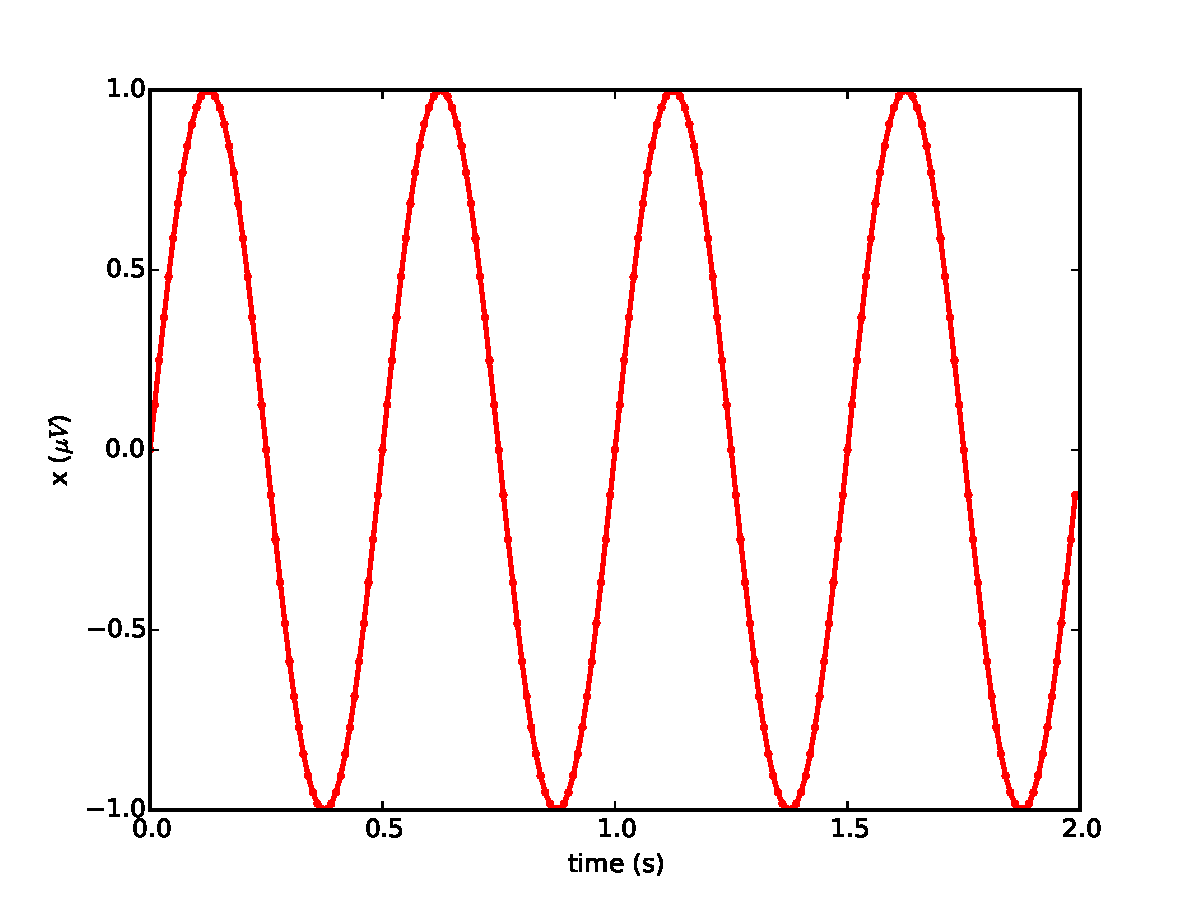
\includegraphics[width=6cm]{./fig/matplotlibSinus.pdf}
\end{center}
\end{frame}
%_______________________________________________________________________________
%_______________________________________________________________________________
\subsubsection{savefig}
%_______________________________________________________________________________
%_______________________________________________________________________________
\begin{frame}[fragile]
\frametitle{Matplotlib}
\framesubtitle{Saving figures}
\begin{itemize}
 \item Sauvegarde manuelle à partir de la fenêtre ouverte sur l'icône save.  
 \item sauvegarde en ligne de commande (savefig) sans passage par un affichage à l'écran.  
\end{itemize}
\begin{pythonConsole}
...
>>> matplotlib.pyplot.ylabel("x ($\mu V$)")
>>> # matplolib.pyplot.show()
>>> matplotlib.pyplot.savefig("./sinus.ps")
>>> matplotlib.pyplot.savefig("./sinus.pdf")
>>> matplotlib.pyplot.savefig("./sinus.svg")
>>> matplotlib.pyplot.savefig("./sinus.tiff")
>>> matplotlib.pyplot.savefig("./sinus.png")
>>> matplotlib.pyplot.savefig("./sinus.jpg")
\end{pythonConsole}
\end{frame}
%_______________________________________________________________________________
%_______________________________________________________________________________
\subsubsection{pylab}
%_______________________________________________________________________________
%_______________________________________________________________________________
\begin{frame}[fragile]
\frametitle{Matplotlib}
\framesubtitle{Pylab}
\begin{itemize}
 \item Fonctions à la Matlab dans le sous-paquet pylab (matplotlib.pylab)
 \item Beaucoup de fonctions sous formes abrégées \dots
\end{itemize}
\begin{minipage}[c]{5cm}
\begin{pythonConsole}
>>> import matplotlib.pylab as mpl
>>> len(dir(mpl))
955

>>> from pylab import *
>>> t = arange(0, 10, 0.01)
>>> f = arange(0, 5, 0.005)
>>> x = sin(2 * pi * f * t)
>>> subplot(2, 1, 1)
>>> plot(t, x * 5)
>>> plot(t, f)
>>> subplot(2, 1, 2)
>>> res = specgram(x, NFFT=64, 
... Fs=100, noverlap=8)
>>> show()
\end{pythonConsole}
\end{minipage}
\begin{minipage}[c]{5cm}
 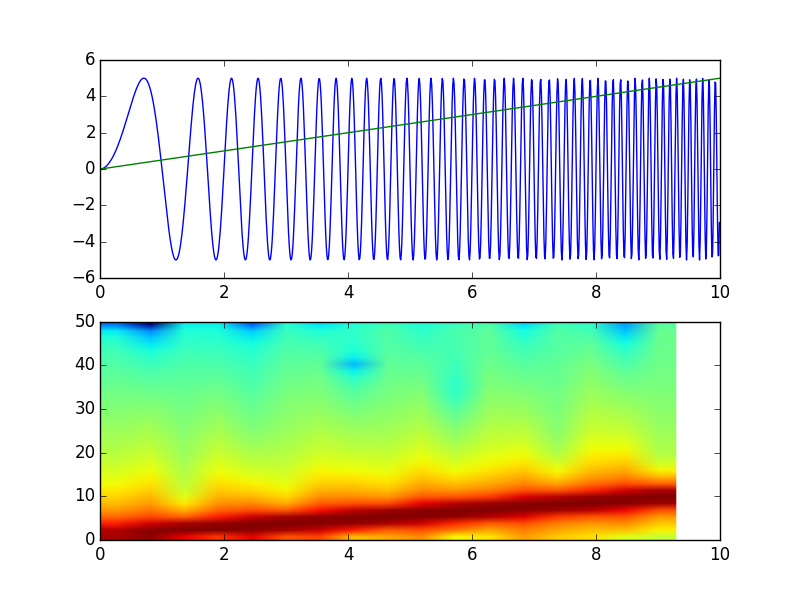
\includegraphics[width=5cm]{./fig/specgram.png}
\end{minipage}
\end{frame}
%_______________________________________________________________________________
%_______________________________________________________________________________
\begin{frame}[fragile]
\frametitle{Matplotlib}
\framesubtitle{Pylab}
\begin{minipage}{5cm}
\begin{pythonConsole}
>>> (X, Y) = meshgrid(linspace(-2, 2, \
... 500), linspace(-2, 2, 500))
>>> Z = X + Y * 1j
>>> for k in range(76): 
...  Z -= (Z / 3 - 1) / (3 * Z ** 2)
>>> close("all")	
>>> imshow(angle(Z))
>>> # savefig('/MonChemin/Lenom.pdf')
>>> show()
\end{pythonConsole}
\end{minipage}
\begin{minipage}{5cm}
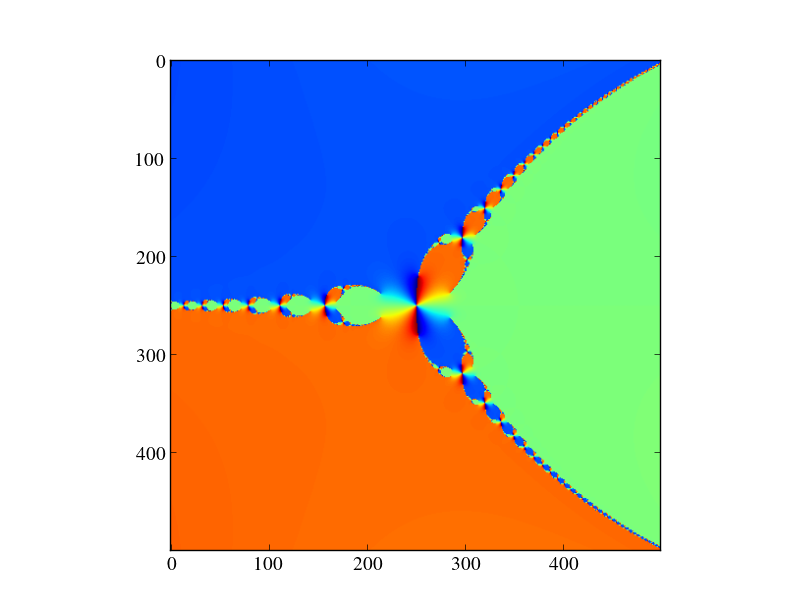
\includegraphics[width=5cm]{fig/fractal.png}
\end{minipage}
\end{frame}
%_______________________________________________________________________________
%_______________________________________________________________________________
\begin{frame}
\frametitle{Matplotlib}
\framesubtitle{Exemples de Nicolas Le Bihan}
\begin{minipage}{0.4\linewidth}
\begin{figure}
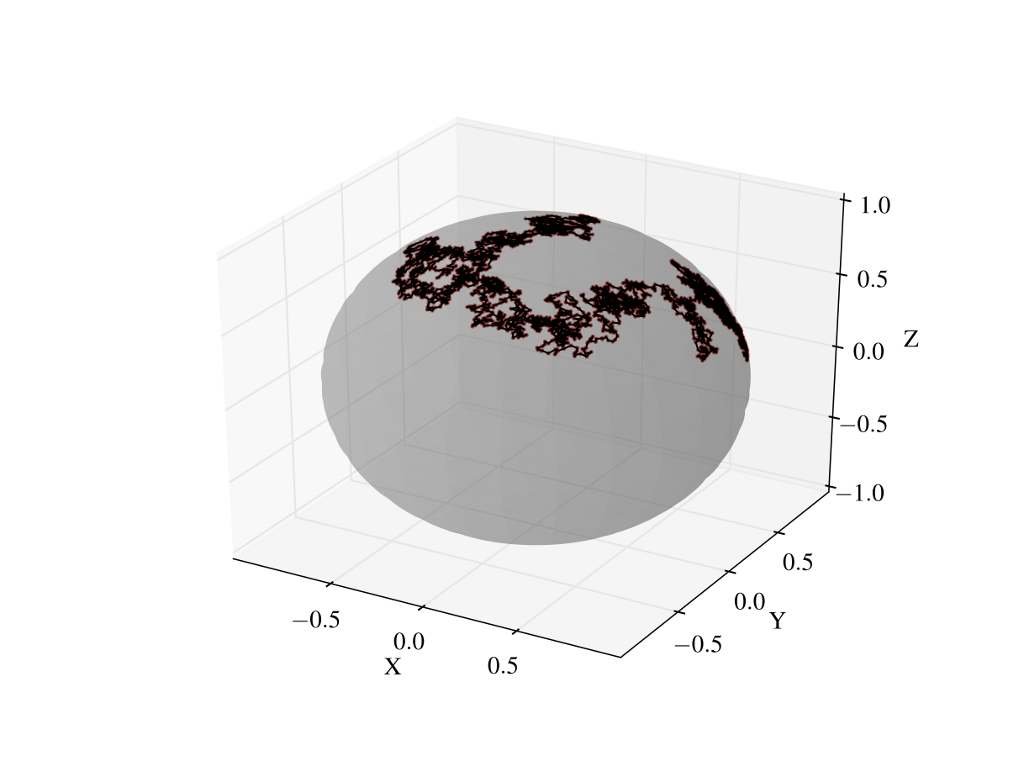
\includegraphics[width=6.5cm,height=5.5cm]{fig/BrownSphere.png}
\end{figure}
\end{minipage}
\hspace{1cm}
\begin{minipage}{0.4\linewidth}
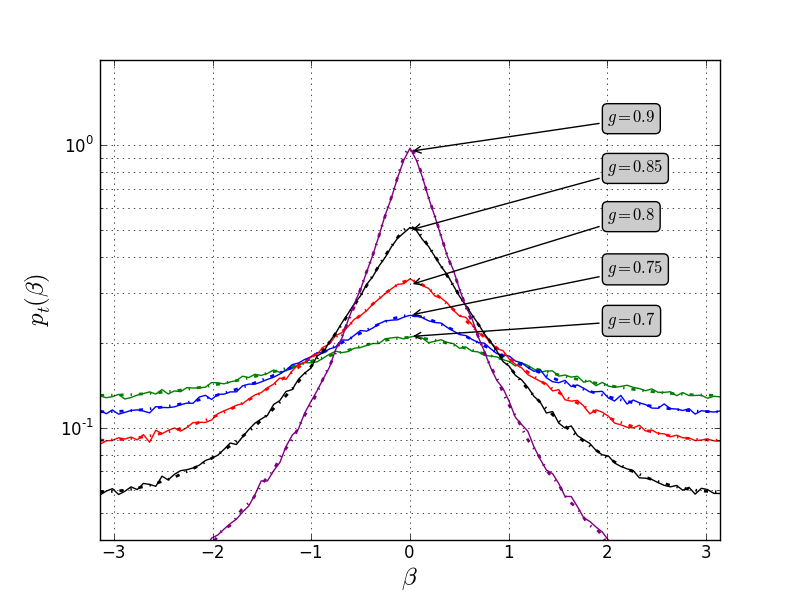
\includegraphics[width=5.5cm,height=4.5cm]{fig/Distrib.png}
\end{minipage}
\end{frame}
%_______________________________________________________________________________
%_______________________________________________________________________________
\subsection{Pandas}
%_______________________________________________________________________________
%_______________________________________________________________________________
\begin{frame}[fragile]
\frametitle{Pandas}
\framesubtitle{}
\begin{itemize}
 \item \myFig{height=0.5cm}{./fig/pandas-logo.png} \, \url{http://www.scipy.org/scipylib/index.html}
 \item \emph{data structure and analysis}
 \item ressemble au traitement de données sous R (data.frame) 
\end{itemize}

\begin{pythonConsole}
>>> import pandas as pd
>>> a = [1., 2., 3., 2., 1., 2., 3., 2., 1]
>>> data = pd.DataFrame(a)
>>> print(a)
   0
0  1
1  2
2  3
3  2
4  1
5  2
6  3
7  2
8  1
\end{pythonConsole}
\end{frame}
%_______________________________________________________________________________
%_______________________________________________________________________________
\begin{frame}[fragile]
\frametitle{Pandas}
\framesubtitle{}
\begin{itemize}
 \item facilité de traitement des données 
\end{itemize}

\begin{pythonConsole}
>>> taille = 170 + 10 * np.random.randn(100)
>>> masse = 70 + 10 * np.random.randn(100)
>>> dico = {'taille': taille, 'masse': masse}
>>> data = pd.DataFrame(dico)
>>> data.describe()
            masse      taille
count  100.000000  100.000000
mean    70.507943  169.915690
std      9.999280   10.264489
min     45.467455  144.149219
25%     63.300037  162.736237
50%     70.043825  171.168028
75%     78.153612  176.164359
max     94.118966  201.781565
\end{pythonConsole}
\end{frame}
%_______________________________________________________________________________
%_______________________________________________________________________________
\begin{frame}[fragile]
\frametitle{Pandas}
\framesubtitle{}
\begin{itemize}
 \item Possibilité d'indexation spéciale.  
\end{itemize}

\begin{pythonConsole}
>>> help(pd.Series)
class Series(Series)
 |  One-dimensional ndarray with axis labels (including time series).
>>> t = np.arange(0, 3, 0.1)
>>> x = np.cos(2 * np.pi * 2 * t)
>>> s = pd.Series(x, t)
>>> print(s[0:0.5])
0.0    1.000000
0.1    0.309017
0.2   -0.809017
0.3   -0.809017
0.4    0.309017
0.5    1.000000
\end{pythonConsole}
\end{frame}
%_______________________________________________________________________________
%_______________________________________________________________________________
\subsection{IPython}
%_______________________________________________________________________________
%_______________________________________________________________________________
\begin{frame}[fragile]
\frametitle{IPython}
\framesubtitle{}
\begin{itemize}
 \item \myFig{height=0.5cm}{./fig/ipython-logo.png} \, \url{http://www.scipy.org/scipylib/index.html}
 \item \emph{Enhanced python console}
 \item Attention, ce n'est pas un paquet mais une console améliorée !
 \item Accessible à partir d'un terminal (ipython) 
 \item Complétion automatique avec la touche tab
 \item Fonctions magiques (magic)
\end{itemize}

\begin{shell}
$ ipython /* $ */
\end{shell} 

\begin{pythonConsole}
Python 2.7.3 | 64-bit | (default, Jun 14 2013, 18:17:36) 
Type "copyright", "credits" £or£ "license" £for£ more information.

IPython 2.2.0 -- An enhanced Interactive Python.
?         -> Introduction £and£ overview of IPython£'£s features.
%quickref -> Quick reference.
help      -> Python£'£s own help system.
object?   -> Details about 'object', use 'object??' £for£ extra details.

In [1]: %pylab
Using matplotlib backend: MacOSX
Populating the interactive namespace £from£ numpy £and£ matplotlib


In [2]: 
\end{pythonConsole}
\end{frame}
%_______________________________________________________________________________
%_______________________________________________________________________________
\subsubsection{ipython notebook}
%_______________________________________________________________________________
%_______________________________________________________________________________
\begin{frame}[fragile]
\frametitle{IPython}
\framesubtitle{ipython notebook}
\begin{itemize}
 \item Accessible à partir d'un terminal (ipython notebook) 
 \item Ouverture et création de notebooks (*.pynb)
\end{itemize}
\begin{center}
 \myFig{width=8cm}{./fig/ipython_notebook_server.png}
\end{center}
\end{frame}
%_______________________________________________________________________________
%_______________________________________________________________________________
\begin{frame}[fragile]
\frametitle{IPython}
\framesubtitle{ipython notebook}
\begin{itemize}
 \item Les cellules exécutent du code ou formatent du texte
 \item Chargement des fonctions pylab avec affichage dans le notebook : \%pylab inline 
\end{itemize}
\begin{center}
 \myFig{width=8cm}{./fig/ipython_notebook_p1.png}
\end{center}
\end{frame}
%_______________________________________________________________________________
%_______________________________________________________________________________
\begin{frame}[fragile]
\frametitle{IPython}
\framesubtitle{ipython notebook}
\begin{itemize}
 \item Saisie et affichage en HTML et LaTeX, entre autres.   
\end{itemize}
\begin{center}
 \myFig{width=8cm}{./fig/ipython_notebook_p2.png}
\end{center}
\end{frame}
%_______________________________________________________________________________
%_______________________________________________________________________________
\subsection{Mayavi}
%_______________________________________________________________________________
%_______________________________________________________________________________
\begin{frame}
\frametitle{Mayavi}
\framesubtitle{}
\frameCC{%
\begin{itemize}
 \item \url{http://docs.enthought.com/mayavi/mayavi}
 \item \url{https://github.com/enthought/mayavi}
 \item Manipulation des objets 3D améliorée (objet vtk). 
\end{itemize}
}
{\myFig{width=8cm}{./fig/Mayavi_site.png}}
\end{frame}
%_______________________________________________________________________________
%_______________________________________________________________________________
\begin{frame}
\frametitle{Mayavi}
\framesubtitle{}
\myFigCentered{width=8cm}{./fig/Mayavi.png}
\end{frame}
%_______________________________________________________________________________
%_______________________________________________________________________________
\begin{frame}[fragile]
\frametitle{Mayavi}
\framesubtitle{import mayavi.engine}
\begin{itemize}
 \item Dans une console Python : import mayavi. \dots
\end{itemize}
\begin{pythonConsole}
>>> from mayavi.api import Engine
>>> engine = Engine()
>>> engine.start()
>>> engine.new_scene()
>>> from mayavi.sources.parametric_surface import ParametricSurface
>>> parametric_surface1 = ParametricSurface()
>>> scene = engine.scenes[0]
>>> engine.add_source(parametric_surface1, scene)
>>> from mayavi.modules.surface import Surface
>>> surface1 = Surface()
>>> engine.add_filter(surface1,parametric_surface1)
\end{pythonConsole}
\end{frame}
%_______________________________________________________________________________
%_______________________________________________________________________________
\subsection{scikit-learn}
%_______________________________________________________________________________
%_______________________________________________________________________________
\begin{frame}[fragile]
\frametitle{Scikit-learn}
\framesubtitle{}
\begin{itemize}
 \item \url{http://scikit-learn.org/} 
 \item \url{https://github.com/scikit-learn/scikit-learn} 
\end{itemize}
\myFigCentered{width=8cm}{./fig/scikit-learn.png}
\end{frame}
%_______________________________________________________________________________
%_______________________________________________________________________________
\begin{frame}[fragile]
\frametitle{Scikit-learn}
\framesubtitle{Help content}
\begin{pythonConsole}
>>> import sklearn
>>> help(sklearn)

DESCRIPTION
    Machine learning module for Python
    ==================================
    
    sklearn £is£ a Python module integrating classical machine
    learning algorithms £in£ the tightly-knit world of scientific Python
    packages (numpy, scipy, matplotlib).
    
    It aims to provide simple £and£ efficient solutions to learning problems
    that are accessible to everybody £and£ reusable £in£ various contexts:
    machine-learning as a versatile tool £for£ science and engineering.
    
    See http://scikit-learn.org £for£ complete documentation.

PACKAGE CONTENTS
    __check_build (package)
    _build_utils
    _hmmc
    _isotonic
    base
    cluster (package)
    covariance (package)
    cross_decomposition (package)
    cross_validation
    datasets (package)
    decomposition (package)
    dummy
    ensemble (package)
    externals (package)
\end{pythonConsole}
\end{frame}
%_______________________________________________________________________________
%_______________________________________________________________________________
\begin{frame}[fragile]
\frametitle{Scikit-learn}
\framesubtitle{Help content}
\begin{pythonConsole}
    feature_extraction (package)
    feature_selection (package)
    gaussian_process (package)
    grid_search
    hmm
    isotonic
    kernel_approximation
    lda
    learning_curve
    linear_model (package)
    kernel_approximation
    lda
    learning_curve
    linear_model (package)
    manifold (package)
    metrics (package)
    mixture (package)
    multiclass
    naive_bayes
    neighbors (package)
    neural_network (package)
    pipeline
    pls
    preprocessing (package)
    qda
    random_projection
    semi_supervised (package)
    setup
    svm (package)
    tests (package)
    tree (package)
    utils (package)
\end{pythonConsole}
\end{frame}
%_______________________________________________________________________________
%_______________________________________________________________________________
\begin{frame}[fragile]
\frametitle{Scikit-learn}
\framesubtitle{Exemple de Classifieur : Linear Discriminant Analysis}
\begin{pythonConsole}
>>> from pylab import *
>>> from sklearn.datasets import load_iris
>>> from sklearn.lda import LDA
>>> dic = load_iris()
>>> x = dic["data"]
>>> y = dic["target"]
>>> nClasses = unique(y).size
>>> clf = LDA()
>>> clf.fit(x[:, :2], y)
>>> (mx1, mx2) = meshgrid(linspace(4, 8, 100), linspace(2, 5, 100))
>>> Z = clf.predict(vstack((mx1.flatten().T, mx2.flatten())).T)
>>> pcolor(mx1, mx2, Z.reshape(mx1.shape), alpha=0.1)
>>> colors = ["b", "g", "r"]
>>> for i in range(nClasses): 
>>>   scatter(x[y==i, 0], x[y==i, 1], c=colors[i])
>>> axis(xmin=4, xmax=8, ymin=2, ymax=5)
>>> show()
\end{pythonConsole}
\myFigCentered{width=4cm}{./fig/sklearn_lda.png}
\end{frame}
%_______________________________________________________________________________
%_______________________________________________________________________________
\subsection{Autres ressources : exemple C}
%_______________________________________________________________________________
\begin{frame}[fragile]
\frametitle{Importation de bibliothèques de fonctions écrites en C}
\framesubtitle{Exemple using module ctypes}
\begin{python}
import ctypes
libName = './clz.lib'
libCLZ = ctypes.CDLL(libName)
clz_c = libCLZ.clz
clz_c.restype = ctypes.c_uint
sequence = numpy.ctypeslib.ndpointer(dtype=numpy.int) 
clz_c.argtypes = ([sequence, ctypes.c_uint])
# conversion of s into sequence with numpy.asarray
c = clz_c(numpy.asarray(s, dtype='int'), n)
\end{python}
\end{frame}
%_______________________________________________________________________________

